%------------------------------------------------------------------------------
\chapter{Störkörpermessung}
\label{sec:stoerkoerpermessung}
%------------------------------------------------------------------------------
\section{Vorbereitung}
\subsection{Vorbereitung}
Abstimmen auf Luft, Symmetrisierung des Feldes

Unterschied Vakuum--Luft \cite{pozar} (S. 308):
\begin{align}
\omega \approx \omega_0 \cdot \frac{3 - \epsilon_\mathrm{r}}{2}
\end{align}
Permittivität Luft (trocken und CO2-frei) \cite{CRC} (S.1093):
\begin{align}
\epsilon_\mathrm{r}^\mathrm{Luft} = \num{1.0005364}
\end{align}




\subsection{Störkörperkonstante}
Berechnung der Störkörperkonstante

PTFE hat verschwindende magnetische Suszeptibilität [QUELLE] und erlaubt die Verwendung vonweshalb Gleichung \eqref{eq:skm_e_feld_normiert} für dielektrische Kugeln zur Bestimmung der Amplitude des elektrischen Feldes im Resonator genutzt werden kann.


Permittivität Teflon \cite{CRC}(S. 2201) $\epsilon_\mathrm{r} = \num{2.1}$.
Berechnen der Störkörperkonstante \todo{Fehler ist noch nicht richtig!}:
\begin{align}
  \alpha_\mathrm{s} = \SI{2.985 +- 0.092e-17}{\ampere\second\metre\squared\per\volt}
\end{align}


\subsection{Messung von Resonanzfrequenz und Güte}
Resonanzfrequenz und Güte (fit)
Messung Güte: Erwärmung des Resonators führt zu einer Verringerung der Leitfähigkeit des Kupfers und somit zu einer Reduzierung der Güte.

\begin{figure}[ht]
  \centering
  % GNUPLOT: LaTeX picture with Postscript
\begingroup
  \makeatletter
  \providecommand\color[2][]{%
    \GenericError{(gnuplot) \space\space\space\@spaces}{%
      Package color not loaded in conjunction with
      terminal option `colourtext'%
    }{See the gnuplot documentation for explanation.%
    }{Either use 'blacktext' in gnuplot or load the package
      color.sty in LaTeX.}%
    \renewcommand\color[2][]{}%
  }%
  \providecommand\includegraphics[2][]{%
    \GenericError{(gnuplot) \space\space\space\@spaces}{%
      Package graphicx or graphics not loaded%
    }{See the gnuplot documentation for explanation.%
    }{The gnuplot epslatex terminal needs graphicx.sty or graphics.sty.}%
    \renewcommand\includegraphics[2][]{}%
  }%
  \providecommand\rotatebox[2]{#2}%
  \@ifundefined{ifGPcolor}{%
    \newif\ifGPcolor
    \GPcolortrue
  }{}%
  \@ifundefined{ifGPblacktext}{%
    \newif\ifGPblacktext
    \GPblacktexttrue
  }{}%
  % define a \g@addto@macro without @ in the name:
  \let\gplgaddtomacro\g@addto@macro
  % define empty templates for all commands taking text:
  \gdef\gplbacktext{}%
  \gdef\gplfronttext{}%
  \makeatother
  \ifGPblacktext
    % no textcolor at all
    \def\colorrgb#1{}%
    \def\colorgray#1{}%
  \else
    % gray or color?
    \ifGPcolor
      \def\colorrgb#1{\color[rgb]{#1}}%
      \def\colorgray#1{\color[gray]{#1}}%
      \expandafter\def\csname LTw\endcsname{\color{white}}%
      \expandafter\def\csname LTb\endcsname{\color{black}}%
      \expandafter\def\csname LTa\endcsname{\color{black}}%
      \expandafter\def\csname LT0\endcsname{\color[rgb]{1,0,0}}%
      \expandafter\def\csname LT1\endcsname{\color[rgb]{0,1,0}}%
      \expandafter\def\csname LT2\endcsname{\color[rgb]{0,0,1}}%
      \expandafter\def\csname LT3\endcsname{\color[rgb]{1,0,1}}%
      \expandafter\def\csname LT4\endcsname{\color[rgb]{0,1,1}}%
      \expandafter\def\csname LT5\endcsname{\color[rgb]{1,1,0}}%
      \expandafter\def\csname LT6\endcsname{\color[rgb]{0,0,0}}%
      \expandafter\def\csname LT7\endcsname{\color[rgb]{1,0.3,0}}%
      \expandafter\def\csname LT8\endcsname{\color[rgb]{0.5,0.5,0.5}}%
    \else
      % gray
      \def\colorrgb#1{\color{black}}%
      \def\colorgray#1{\color[gray]{#1}}%
      \expandafter\def\csname LTw\endcsname{\color{white}}%
      \expandafter\def\csname LTb\endcsname{\color{black}}%
      \expandafter\def\csname LTa\endcsname{\color{black}}%
      \expandafter\def\csname LT0\endcsname{\color{black}}%
      \expandafter\def\csname LT1\endcsname{\color{black}}%
      \expandafter\def\csname LT2\endcsname{\color{black}}%
      \expandafter\def\csname LT3\endcsname{\color{black}}%
      \expandafter\def\csname LT4\endcsname{\color{black}}%
      \expandafter\def\csname LT5\endcsname{\color{black}}%
      \expandafter\def\csname LT6\endcsname{\color{black}}%
      \expandafter\def\csname LT7\endcsname{\color{black}}%
      \expandafter\def\csname LT8\endcsname{\color{black}}%
    \fi
  \fi
    \setlength{\unitlength}{0.0500bp}%
    \ifx\gptboxheight\undefined%
      \newlength{\gptboxheight}%
      \newlength{\gptboxwidth}%
      \newsavebox{\gptboxtext}%
    \fi%
    \setlength{\fboxrule}{0.5pt}%
    \setlength{\fboxsep}{1pt}%
\begin{picture}(6802.00,4534.00)%
    \gplgaddtomacro\gplbacktext{%
      \csname LTb\endcsname%
      \put(814,704){\makebox(0,0)[r]{\strut{}0{,}0}}%
      \csname LTb\endcsname%
      \put(814,1417){\makebox(0,0)[r]{\strut{}0{,}2}}%
      \csname LTb\endcsname%
      \put(814,2130){\makebox(0,0)[r]{\strut{}0{,}4}}%
      \csname LTb\endcsname%
      \put(814,2843){\makebox(0,0)[r]{\strut{}0{,}6}}%
      \csname LTb\endcsname%
      \put(814,3556){\makebox(0,0)[r]{\strut{}0{,}8}}%
      \csname LTb\endcsname%
      \put(814,4269){\makebox(0,0)[r]{\strut{}1{,}0}}%
      \csname LTb\endcsname%
      \put(1835,484){\makebox(0,0){\strut{}499{,}48}}%
      \csname LTb\endcsname%
      \put(3200,484){\makebox(0,0){\strut{}499{,}50}}%
      \csname LTb\endcsname%
      \put(4565,484){\makebox(0,0){\strut{}499{,}52}}%
      \csname LTb\endcsname%
      \put(5930,484){\makebox(0,0){\strut{}499{,}54}}%
    }%
    \gplgaddtomacro\gplfronttext{%
      \csname LTb\endcsname%
      \put(176,2486){\rotatebox{-270}{\makebox(0,0){\strut{}Reflektionskoeffizient $|\rho|$}}}%
      \put(3675,154){\makebox(0,0){\strut{}Frequenz $\nu$ / \si{MHz}}}%
      \csname LTb\endcsname%
      \put(5418,1097){\makebox(0,0)[r]{\strut{}Messpunkte}}%
      \csname LTb\endcsname%
      \put(5418,877){\makebox(0,0)[r]{\strut{}Anpassung}}%
    }%
    \gplbacktext
    \put(0,0){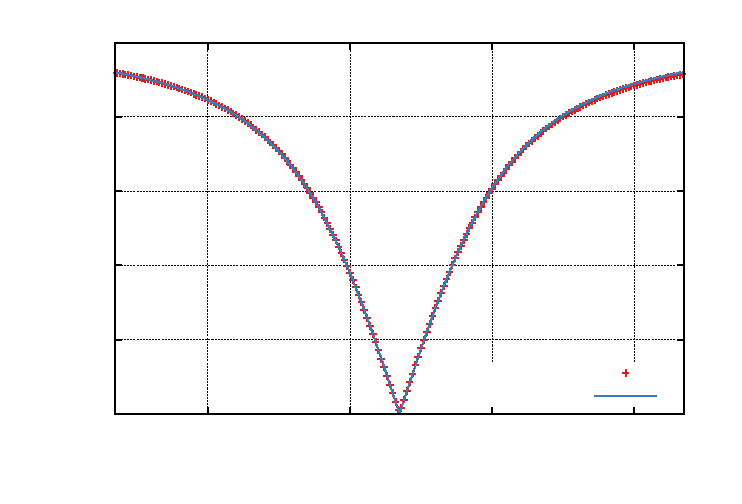
\includegraphics{./plots/guete_fit_pi}}%
    \gplfronttext
  \end{picture}%
\endgroup

  \caption{Gütefit}
  \label{fig:gütefit}
\end{figure}

Ergebnisse des Fits:
\begin{align}
\kappa &= \num{1.01285 +- 0.00091}\\
Q_0 &= \num{29560 +- 13}\\
\nu_0 &= \SI{499.507 +- 0.001}{MHz}
\end{align}

\section{Vermessung der TM010 Beschleunigermode}
Berechnung des elektrischen Feldes\\
Berechnung der charakteristischen Größen des Resonators: Beschleunigungsspannung, Shuntimpedanz und Laufzeitfaktor

Alle anderen Moden (5/6, 1/2, 1/6) haben verschwindende Felder in der zentralen Zelle und können damit nicht gekoppelt werden.

Längenmessung vom Flansch erklären.


\section{Vermessung von Moden höherer Ordnung (PETRA-III)}
